%% LaTeX2e class for student theses
%% sections/evaluation.tex
%% 
%% Karlsruhe Institute of Technology
%% Institute for Program Structures and Data Organization
%% Chair for Software Design and Quality (SDQ)
%%
%% Dr.-Ing. Erik Burger
%% burger@kit.edu
%%
%% Version 1.3.3, 2018-04-17

\chapter{Evaluation}
\label{ch:Evaluation}

In this chapter we will be comparing our algorithm without splitting with the typical light sampling strategy power sampling that creates a light distribution according to the energy of the emitters on different scenes. We are including scenes with point light sources, spotlights and area light sources and also combinations of these light sources. All scenes were rendered on a computer with a Intel® Core™ i7-4770K processor and 16 gigabyte of main memory. The framework used was PBRT version 3 by Pharr, Jakob and Humphreys. \cite{PBRT}

\section{20 spot lights}

\begin{figure}
	\centering
	\begin{subfigure}{.5\textwidth}
		\centering
		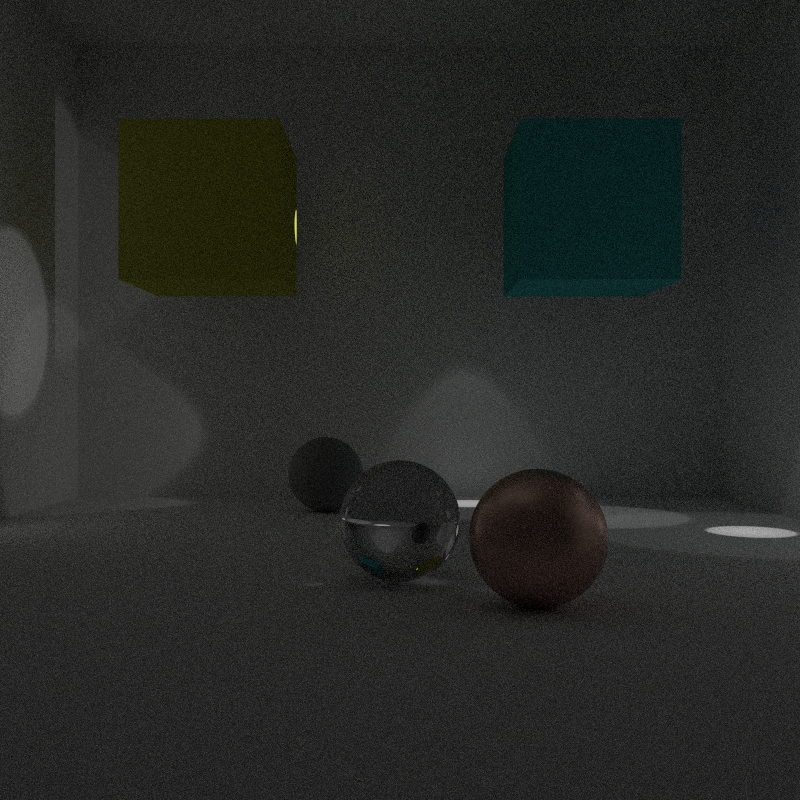
\includegraphics[width=0.95\linewidth]{spotlight_same_direction_64_143s.png}
		\caption{Our algorithm, 64 samples}
		\label{fig:spot1}
	\end{subfigure}%
	\begin{subfigure}{.5\textwidth}
		\centering
		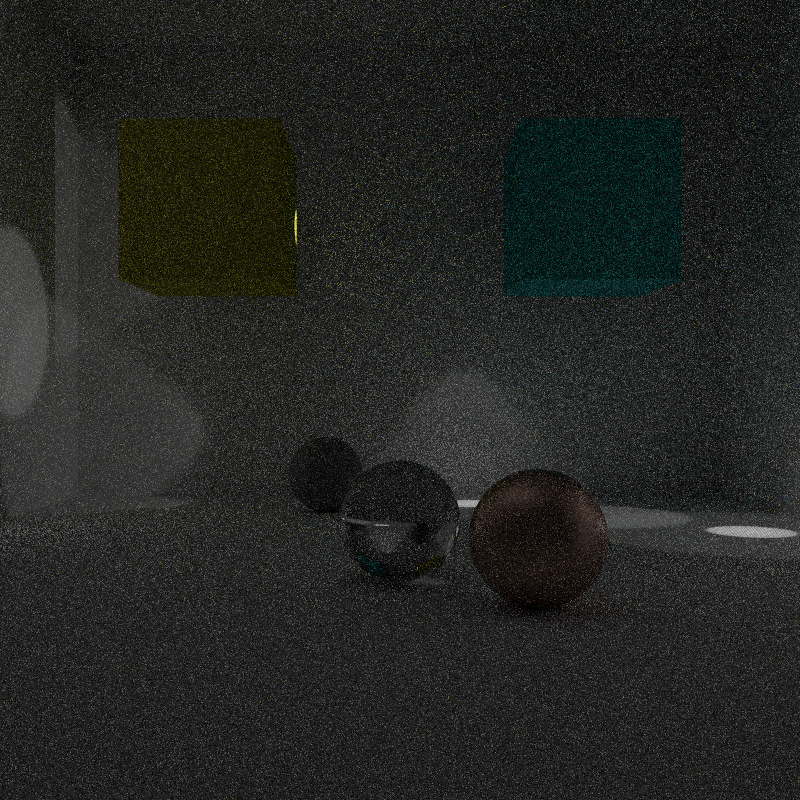
\includegraphics[width=0.95\linewidth]{spotlight_same_direction_old_100_153s.png}
		\caption{Power sampling, 100 samples}
		\label{fig:spot2}
	\end{subfigure}
	\caption{20 spotlights}
	\label{fig:spot}
\end{figure}

First, we wanted to show a scene with very few light sources (\ref{fig:spot}). This scene is only lighted by 20 spotlights that we put in the scene. Both were rendered in about 150 seconds. As we can see, even with very small numbers of emitters, our algorithm leads to a much better image quality.

\section{1.6 million point light sources on the ceiling}

\begin{figure}
	\begin{center}
		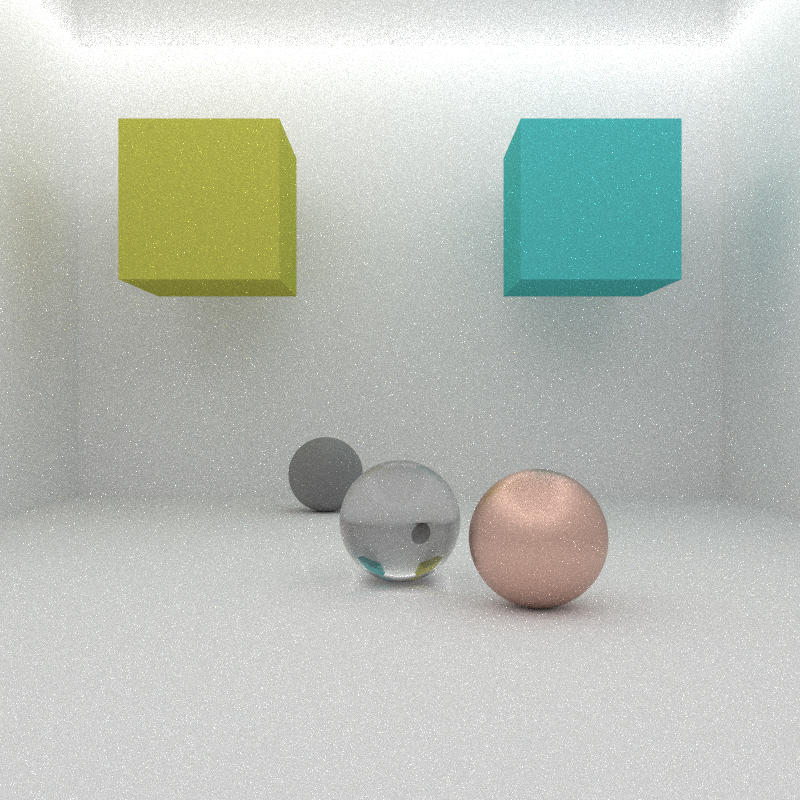
\includegraphics[width=0.8\textwidth]{point_ceil_64_230s.png}
		\caption{1.6 million point lights on the ceiling}
		\label{fig:many}
	\end{center}
\end{figure}

This scene (\ref{fig:many}) uses about 1.6 million point light sources that are offset by a bit at the ceiling of the room and covering the complete surface of the ceiling. The point lights are ordered in a 2D-raster with identical distance. The rendering time of this scene was 230 seconds, while the same scene with a single area light source that covered the whole ceiling
is about 3 times faster with a rendering time of 73 seconds. That proves that our algorithm does indeed scale very well with many emitters because we will rarely find a scene with more than 1.6 million light sources.

\section{12.000 point light sources in a 3D-raster covering the whole room}

\begin{figure}
	\centering
	\begin{subfigure}{.5\textwidth}
		\centering
		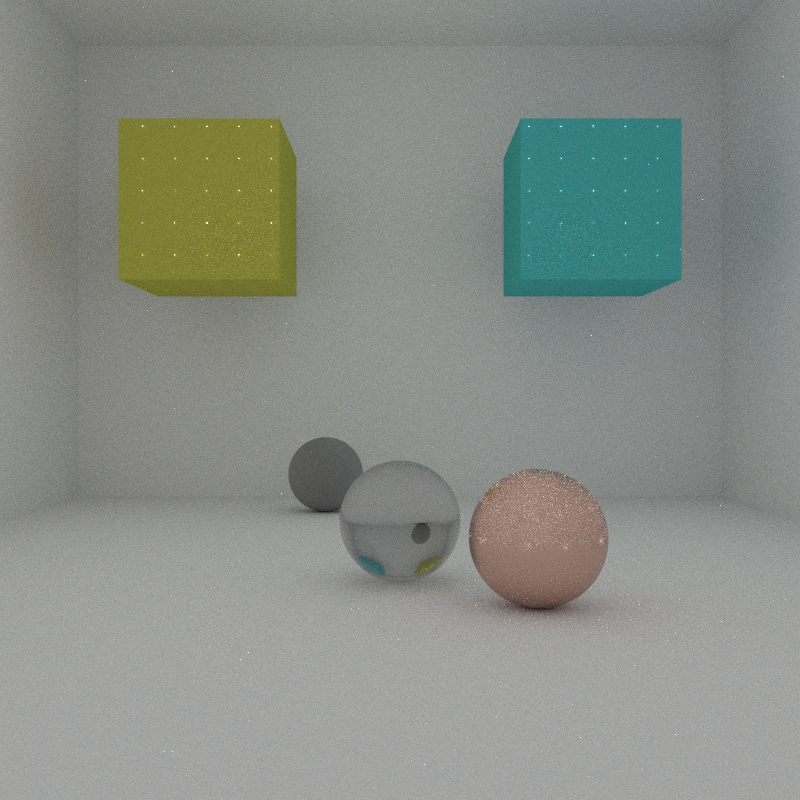
\includegraphics[width=0.95\linewidth]{point_many_32_167s.png}
		\caption{Our algorithm, 32 samples}
		\label{fig:point1}
	\end{subfigure}%
	\begin{subfigure}{.5\textwidth}
		\centering
		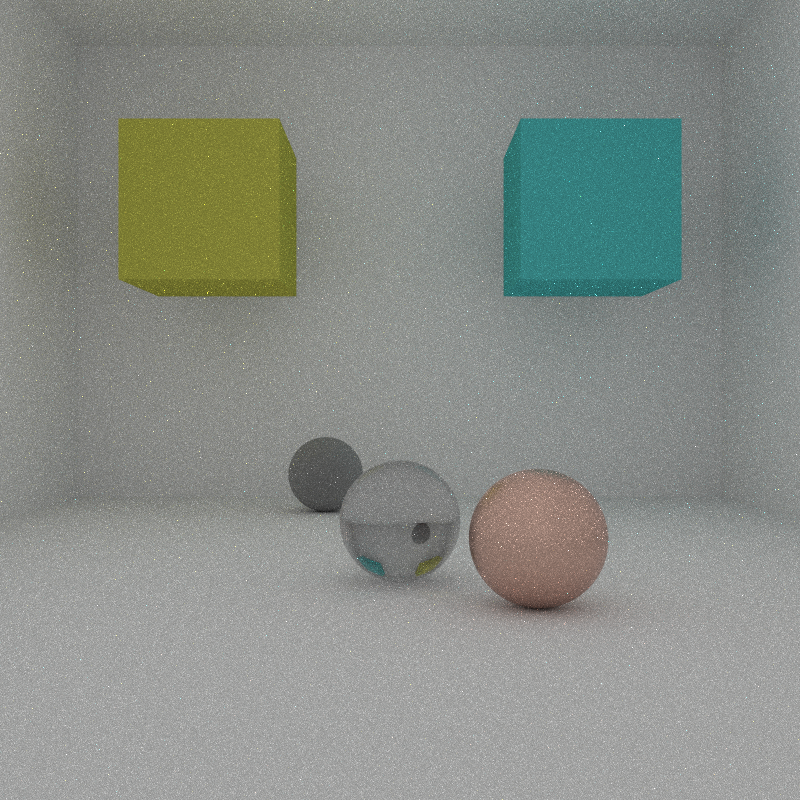
\includegraphics[width=0.95\linewidth]{point_many_90_180s_old.png}
		\caption{Power sampling, 90 samples}
		\label{fig:point2}
	\end{subfigure}
	\caption{12.000 point lights in a 3D-raster}
	\label{pointl}
\end{figure}

This scene (\ref{pointl}) is lighted by 12.000 point light sources that are organized in a 3D-raster. Both images \ref{fig:point1} and \ref{fig:point2} are rendered with similar rendering times of about 170 seconds. The raster covers the whole room with only a bit of space left on the edge of the room. Note, that the small illuminated spots you can see on the boxes in \ref{fig:point1} come from point lights that are very close to the surfaces of the boxes. Using power sampling, the probability of sampling that single light that has a high distribution to the surface is very unlikely and thus, you cannot see these dots while using power sampling. Also, our algorithm produces an image with an objectively better image quality.

\section{12.000 point light sources randomly distributed}

\begin{figure}
	\centering
	\begin{subfigure}{.5\textwidth}
		\centering
		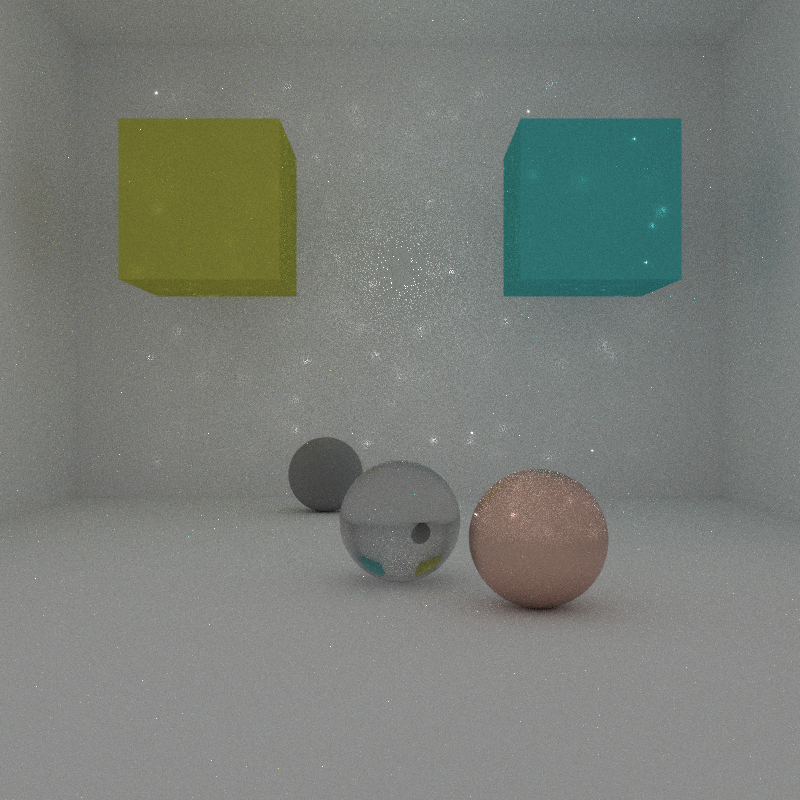
\includegraphics[width=0.95\linewidth]{point_many_ran_32_163s.png}
		\caption{Our algorithm, 32 samples}
		\label{fig:point3}
	\end{subfigure}%
	\begin{subfigure}{.5\textwidth}
		\centering
		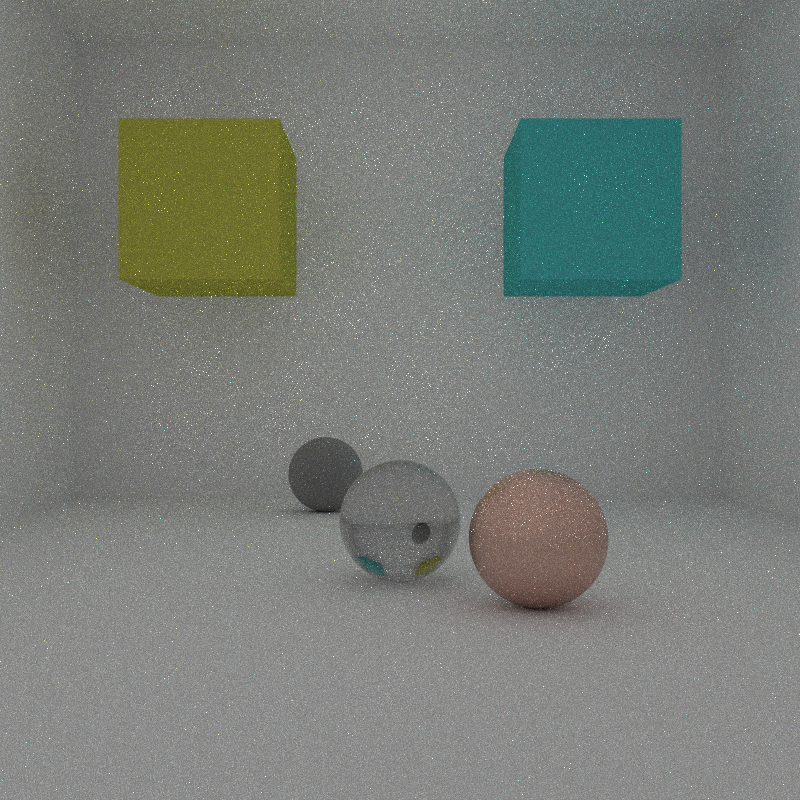
\includegraphics[width=0.95\linewidth]{point_many_ran_old_90_190s.png}
		\caption{Power sampling, 90 samples}
		\label{fig:point4}
	\end{subfigure}
	\caption{12.000 point lights randomly distributed}
	\label{point}
\end{figure}

This scene (\ref{point}) is lighted by 12.000 point light sources that were randomly distributed over the whole room. Both images \ref{fig:point1} and \ref{fig:point2} are rendered with similar rendering times of about 170 seconds. Similar effects like in the scene before can be seen: Our algorithm leads to images with illuminated dots in some places where the light sources were very close to the surface, while the power sampling technique does not. Again, our algorithm produces a less noisy image with a better overall image quality.

\section{12.000 spotlights randomly distributed}

\begin{figure}
	\centering
	\begin{subfigure}{.5\textwidth}
		\centering
		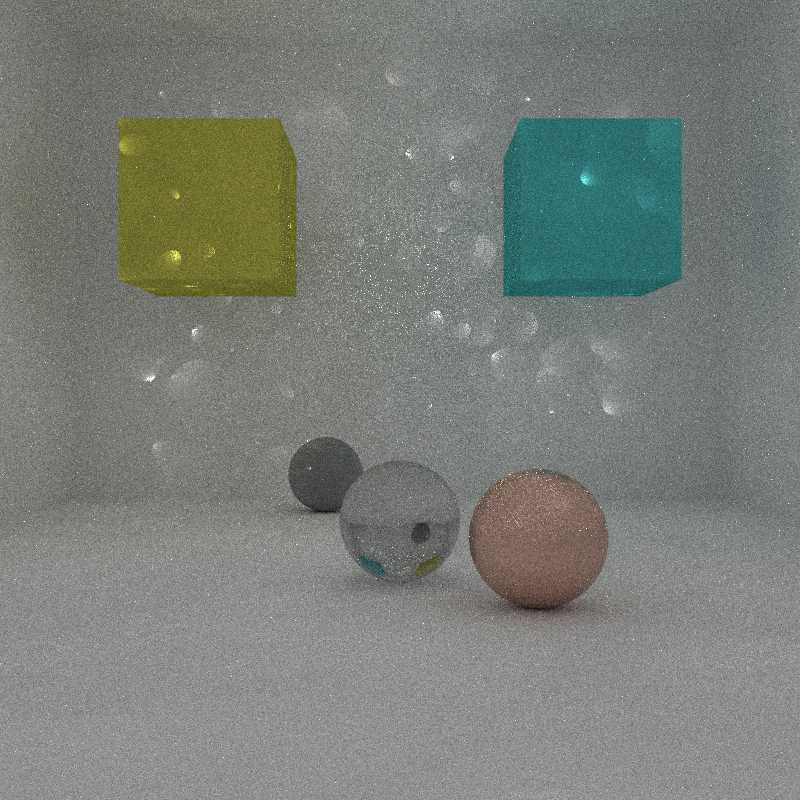
\includegraphics[width=0.95\linewidth]{spotlight_many_64_300s}
		\caption{Our algorithm, 32 samples}
		\label{fig:spot3}
	\end{subfigure}%
	\begin{subfigure}{.5\textwidth}
		\centering
		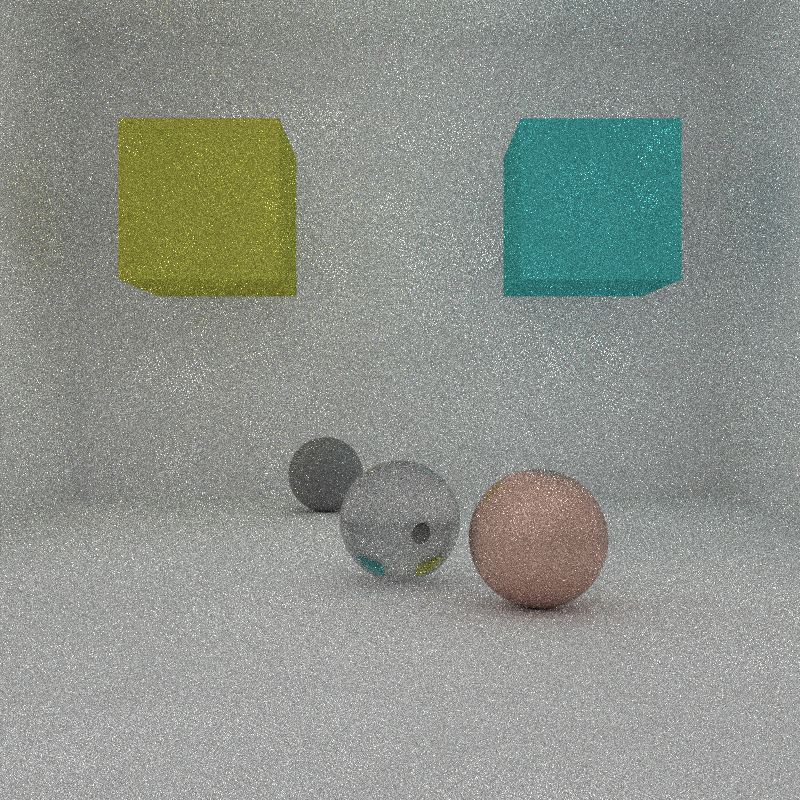
\includegraphics[width=0.95\linewidth]{spotlight_many_old_190_320s}
		\caption{Power sampling, 90 samples}
		\label{fig:spot4}
	\end{subfigure}
	\caption{12.000 spotlights randomly distributed}
	\label{fig:spotl}
\end{figure}

This scene (\ref{fig:spotl}) is lighted by 12.000 spotlights with random position, orientation and aperture angle. Noticeable again are the effects we mentioned earlier, when a light source is close to the surface. Our algorithm again renders an image with a better quality.

\section{2.000 area lights covering the ceiling}

\begin{figure}
	\centering
	\begin{subfigure}{.5\textwidth}
		\centering
		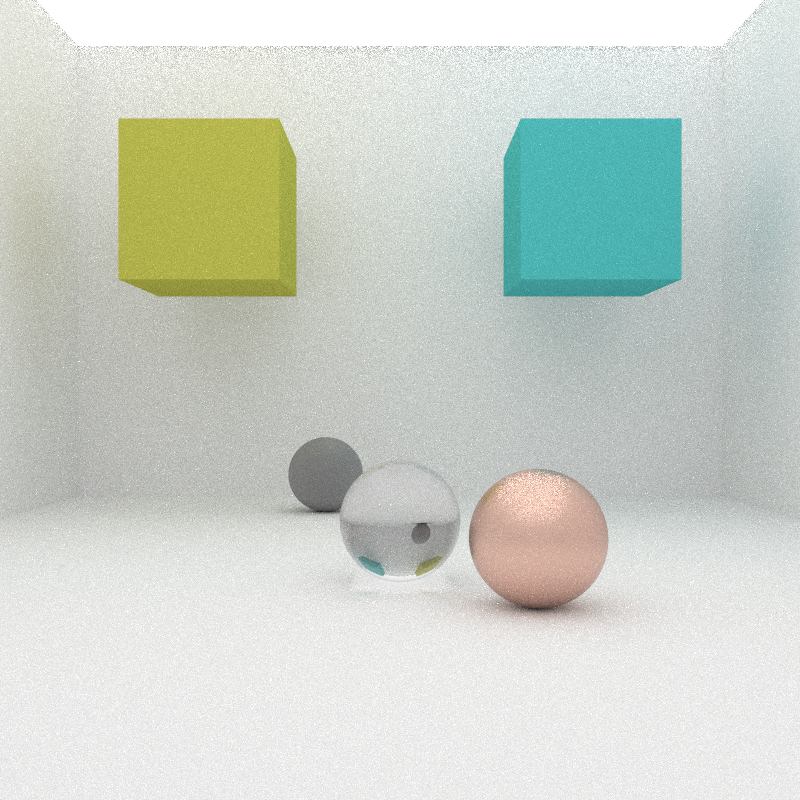
\includegraphics[width=0.95\linewidth]{area_many_64_220s.png}
		\caption{Our algorithm, 64 samples}
		\label{fig:area1}
	\end{subfigure}%
	\begin{subfigure}{.5\textwidth}
		\centering
		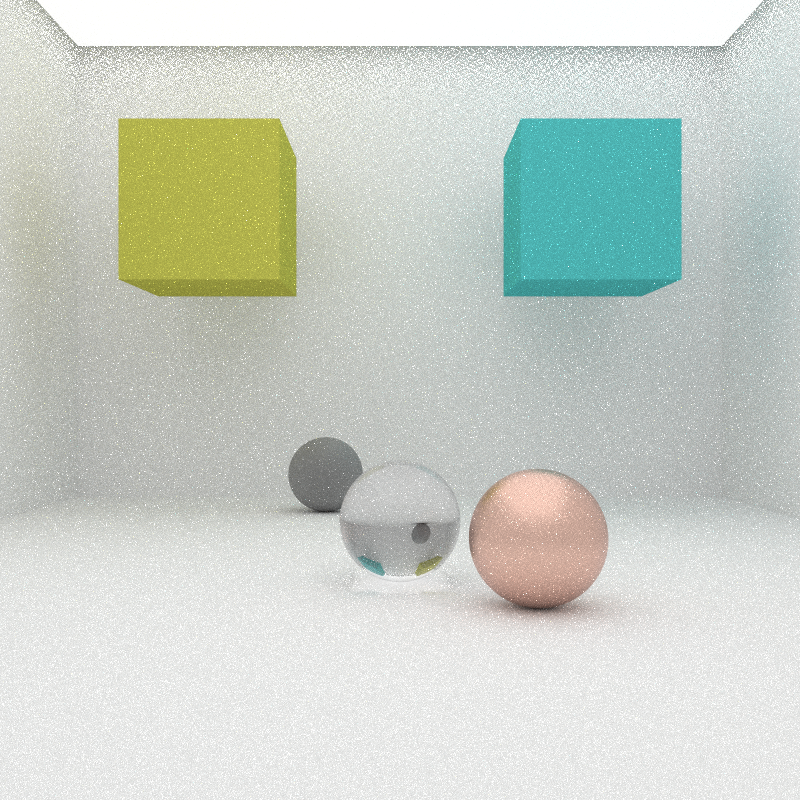
\includegraphics[width=0.95\linewidth]{area_many_old_160_234s.png}
		\caption{Power sampling, 160 samples}
		\label{fig:area2}
	\end{subfigure}
	\caption{2.000 area lights covering the ceiling}
	\label{fig:area}
\end{figure}

This scene (\ref{fig:area}) is lighted by about 2.000 triangle emitters on the ceiling of the room. Especially at the edges around the ceiling, our algorithms yields much better, less noisy results.

\section{6.000 triangle emitters shaping 3 spheres}

\begin{figure}
	\centering
	\begin{subfigure}{.5\textwidth}
		\centering
		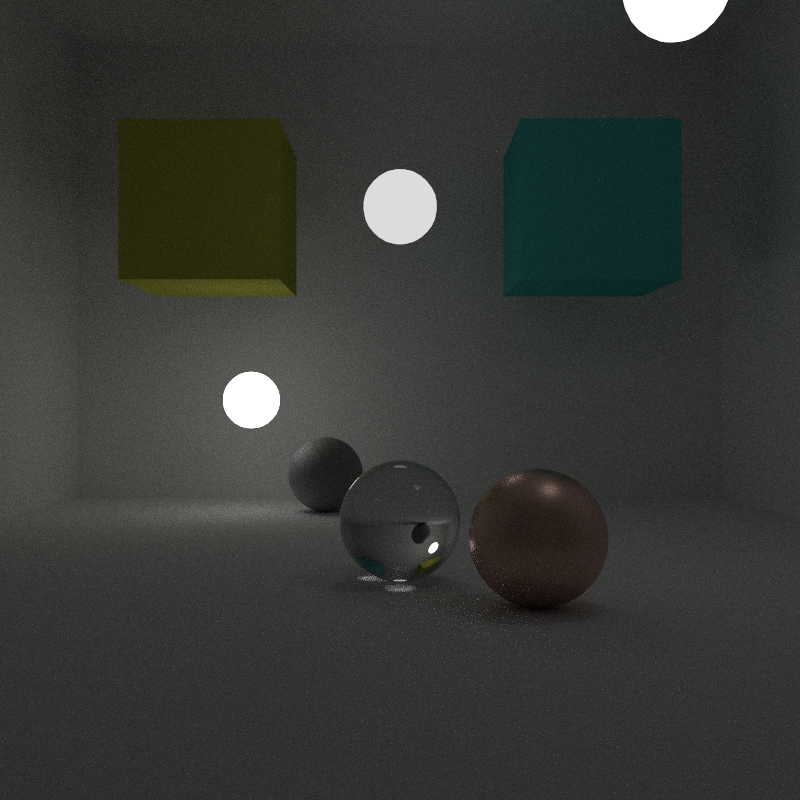
\includegraphics[width=0.95\linewidth]{area_many_sphere_32_160s.png}
		\caption{Our algorithm, 32 samples}
		\label{fig:area3}
	\end{subfigure}%
	\begin{subfigure}{.5\textwidth}
		\centering
		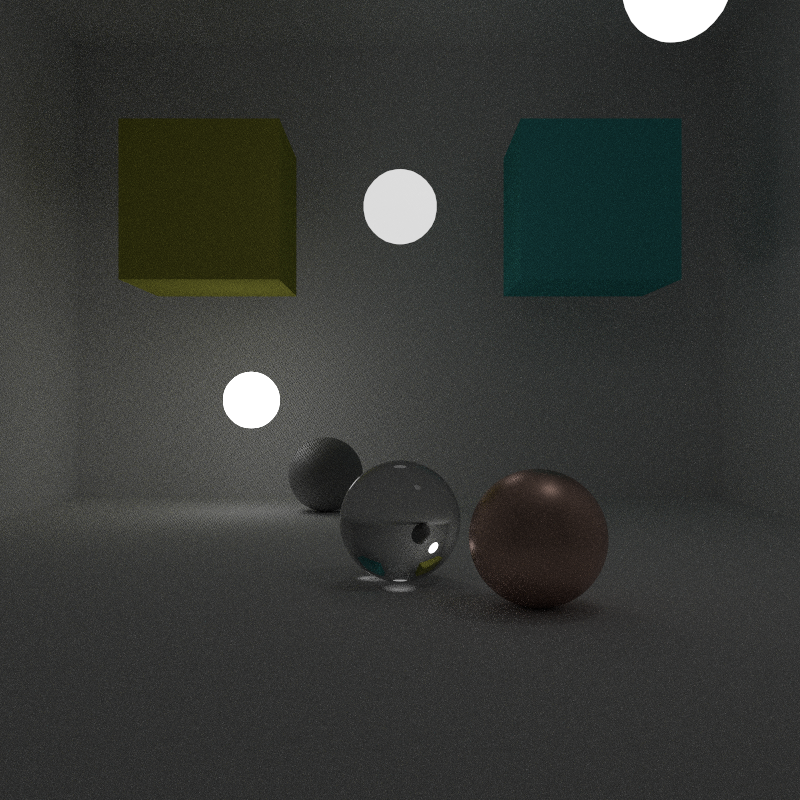
\includegraphics[width=0.95\linewidth]{area_many_sphere_old_75_168s.png}
		\caption{Power sampling, 75 samples}
		\label{fig:area4}
	\end{subfigure}
	\caption{2.000 area lights covering the ceiling}
	\label{fig:areal}
\end{figure}

This scene (\ref{fig:areal}) is lighted by 3 spheres that each consists of 2.000 triangle emitters. Again, you can see the difference in overall image quality. But, in the image we rendered with our algorithm, you can see small blight dots behind the glass sphere. The reason for that is that transmissions of mediums like glass is not covered by our algorithm. If we were to use a higher sampling number, these dots would disappear.

\section{Mixed scene with 6.000 triangle emitters, 4.000 spotlights and 4.000 point lights}

\begin{figure}
	\centering
	\begin{subfigure}{.5\textwidth}
		\centering
		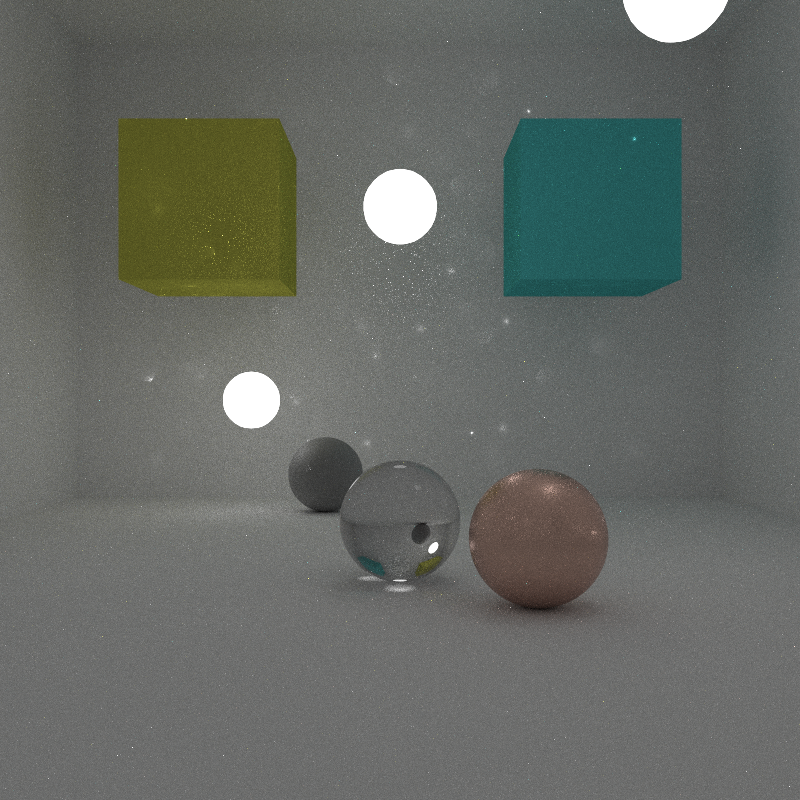
\includegraphics[width=0.95\linewidth]{everything_64_320s.png}
		\caption{Our algorithm, 64 samples}
		\label{fig:every1}
	\end{subfigure}%
	\begin{subfigure}{.5\textwidth}
		\centering
		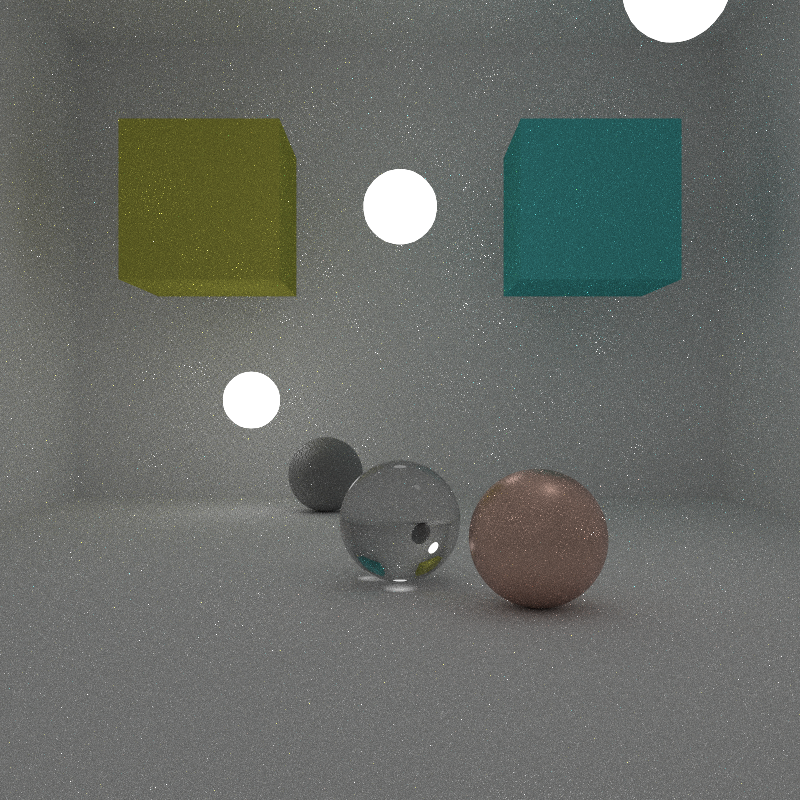
\includegraphics[width=0.95\linewidth]{everything_old_150_330s.png}
		\caption{Power sampling, 150 samples}
		\label{fig:every2}
	\end{subfigure}
	\caption{Mixed scene}
	\label{fig:every}
\end{figure}

This scene consists of the 3 spheres from the previous scene, as well as 4.000 spotlights and point lights randomly distributed over the room. Again, there is not much to say other than that our algorithm creates a less noisy image.

\section{Splitting versus not splitting}

Kulla and Conty \Cite{MLS} showed us that splitting can improve the quality of the rendered image in some scenes drastically. Sadly, we were not able to reproduce the effects on the overall image quality that has been described in their presentation.

\begin{figure}
	\centering
	\begin{subfigure}{.5\textwidth}
		\centering
		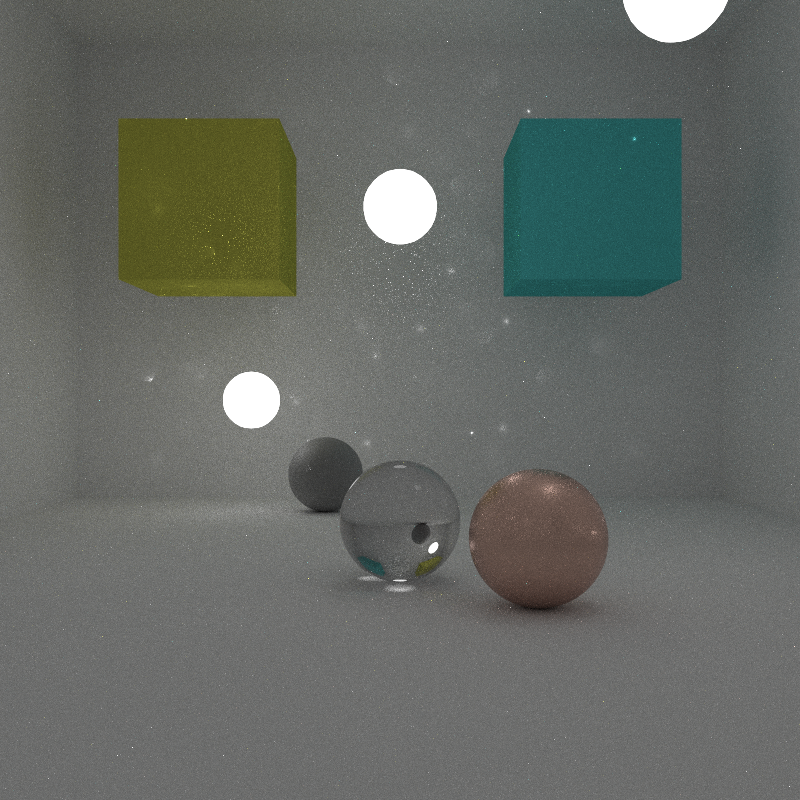
\includegraphics[width=0.95\linewidth]{everything_64_320s.png}
		\caption{No split, 64 samples}
		\label{fig:every3}
	\end{subfigure}%
	\begin{subfigure}{.5\textwidth}
		\centering
		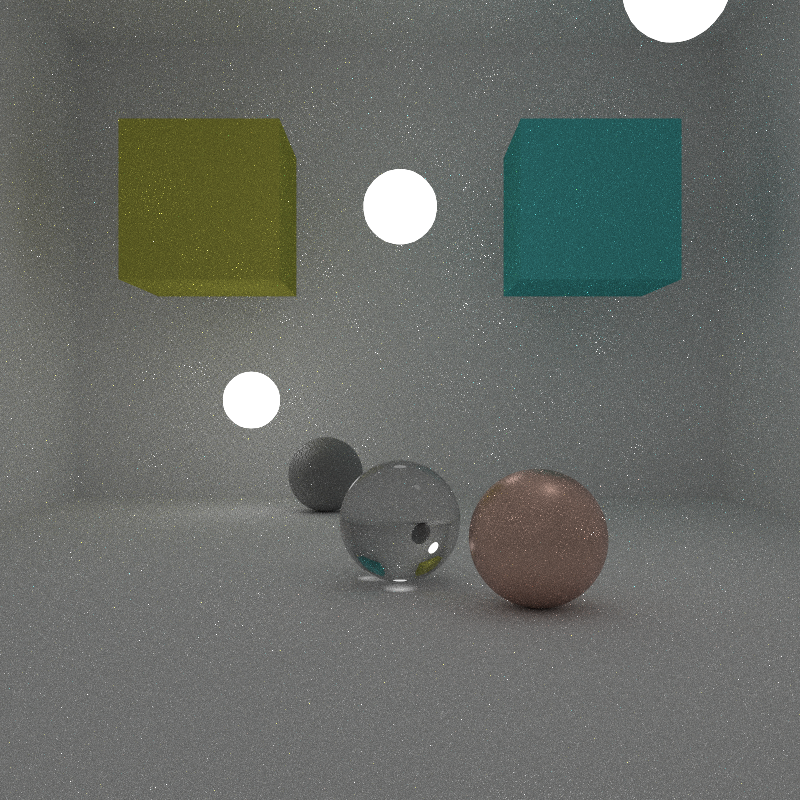
\includegraphics[width=0.95\linewidth]{everything_old_150_330s.png}
		\caption{Split, 32 samples}
		\label{fig:every4}
	\end{subfigure}
	\caption{Mixed scene}
	\label{fig:everyt}
\end{figure}

These two images (\ref{fig:everyt}) were rendered with the previous scenes with and without splitting. The image quality is pretty close but overall a bit better when using no splits. We think that our algorithms still has some issues that we need to address before our splitting algorithm will yield the desirable quality.